%- HandOut Flag -----------------------------------------------------------------------------------------
\newif\ifHandout

%- D0cum3nt ----------------------------------------------------------------------------------------------
\documentclass[beamer,10pt]{standalone}   
%\documentclass[beamer,10pt,handout]{standalone}  \Handouttrue  

%- HandOut Flag -----------------------------------------------------------------------------------------
\ifHandout
	\setbeameroption{show notes} %print notes   
\fi

	
%- Packages ----------------------------------------------------------------------------------------------
\usepackage{custom-style}
\usetikzlibrary{positioning}
\usepackage{multicol}


%--Beamer Style-----------------------------------------------------------------------------------------------
\usetheme{toninus}
\usepackage{animate}
\usetikzlibrary{positioning, arrows}
\usetikzlibrary{shapes}
\usepackage{ifthen}

\begin{document}
%-------------------------------------------------------------------------------------------------------------------------------------------------
\begin{frame}{Phase Space}
\begin{columns}[T]
	\begin{column}{0.5\textwidth}
		\begin{center}
			\resizebox{\textwidth}{!}{		
				\pgfmathtruncatemacro\steps{50}
				\pgfmathtruncatemacro\maxtheta{30}
				\pgfmathtruncatemacro\pi{3.14}
				\begin{animateinline}[autoplay,loop]{10} % 5 fps, same as 0.2 s transduration
				  \multiframe{\steps}{i=0+1}{
				    \begin{tikzpicture}
				    \pgfmathsetmacro\fraction{\i/(\steps-1)}
					\pgfmathsetmacro\theta{\maxtheta*cos(360*\fraction)-90}
					\pgfmathsetmacro\v{-1*sin(360*\fraction)}
				
				    %frame
				    \draw[draw=none] (-6,-8) rectangle (6,6);		
					% Support
					\coordinate (o) at (0,0);
					\node[cross out,draw,black!10] (0,0){};
					\node[circle,draw,black!10] (0,0){};
					% Bob's trajectory
					\draw[blue,line width=1mm] (0,0) circle (4);
					% Rod + Bob
					\draw[dashed] (0,0) -- (\theta:4) node[fill,circle,red](m){};

					% Velocity
					\ifthenelse{\equal{\i}{0}}
           			{}
           			{\draw[-latex,green!80!black,line width=1mm] (m) -- node[green!80!black,below right]{$\vec{v}$}($(m)!\v!-90:(o)$);}
				    \end{tikzpicture}
				  }
				\end{animateinline}
			}
		\end{center}
	\end{column}
	\begin{column}{0.5\textwidth}
		\begin{itemize}
			\item Knowing the position is not sufficient to determine the evolution of the system.
			\item (Displacement encode statics, one must know how configurations evolves in time)
			\item One needs to know also the velocity (or better, the momentum).
		\end{itemize}

		\vspace{1em}
		\onslide<2->{
			\begin{upshotblocksimp}
				Upshot:
				Configurations $\neq$ \emph{States}
			\end{upshotblocksimp}			
		}
	\end{column}
\end{columns}
\end{frame}
\note[itemize]{
	\item
}
%-------------------------------------------------------------------------------------------------------------------------------------------------

%-------------------------------------------------------------------------------------------------------------------------------------------------
\begin{frame}{Phase Space}
\begin{columns}[T]
	\begin{column}{0.5\textwidth}
		\begin{center}
			\resizebox{\textwidth}{!}{
				\begin{tikzpicture}
					\node[draw=none] (o) at (0, 0) {o};
				    %frame
				    \draw[draw=none] (-6,-8) rectangle (6,6);				
					\draw[draw=none](0,0)--(-90:4)node[circle, fill, minimum size=5pt,
				              inner sep=0pt, outer sep=0pt](p){};
					\draw[green,line width=1mm] ($ (p)!3.5cm!90:(o) $) -- ($ (p)!3.5cm!270:(o) $);
					\draw[green,dashed,line width=1mm] ($ (p)!4.5cm!90:(o) $) -- ($ (p)!4.5cm!270:(o) $);
					\draw[blue,line width=1mm] (0,0) circle (4);
				\end{tikzpicture}
			}
			%
		\end{center}
	\end{column}
	\begin{column}{0.5\textwidth}
 		\begin{itemize}
 			\item consider {\bf a} configuration.
 			\item all possible velocities are encoded by points on the tangent line at the given configuration \\(\emph{Tangent space}).
 		\end{itemize}
	\end{column}
\end{columns}
\end{frame}
\note[itemize]{
	\item
}
%-------------------------------------------------------------------------------------------------------------------------------------------------

%-------------------------------------------------------------------------------------------------------------------------------------------------
\begin{frame}{Phase Space}
\begin{columns}[T]
	\begin{column}{0.5\textwidth}
		\begin{center}
			\only<1>{
			\resizebox{\textwidth}{!}{
				\begin{tikzpicture}
					\node[draw=none] (o) at (0, 0) {o};
				    %frame
				    \draw[draw=none] (-6,-8) rectangle (6,6);						
					\foreach \x in {0,30,...,360}{
						\draw[draw=none](0,0)--(\x:4)node[circle, fill, minimum size=5pt,
					              inner sep=0pt, outer sep=0pt](p){};
					\draw[green,line width=1mm] ($ (p)!3.5cm!90:(o) $) -- ($ (p)!3.5cm!270:(o) $);
					\draw[green,dashed,line width=1mm] ($ (p)!4.5cm!90:(o) $) -- ($ (p)!4.5cm!270:(o) $);
					}
						\draw[blue,line width=1mm] (0,0) circle (4);
				\end{tikzpicture}
			}}
			%
			\only<2->{
			\resizebox{.7\textwidth}{!}{
				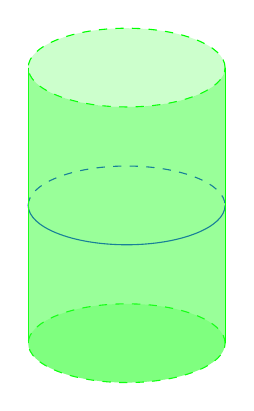
\begin{tikzpicture}
					\draw[green,dashed,fill=green!20] (0,0) ellipse (1.25 and 0.5);
					\draw [blue](-1.25,-1.75) arc (180:360:1.25 and 0.5);
					%\draw [blue,dashed] (-1.25,-3.5) arc (180:360:1.25 and -0.5);
					\draw[green,dashed,fill=green!20] (0,-3.5) ellipse (1.25 and 0.5);
					\draw [blue,dashed] (-1.25,-1.75) arc (180:360:1.25 and -0.5);
					\draw [green](-1.25,0) -- (-1.25,-3.5);
					\draw [green](1.25,-3.5) -- (1.25,0);  
					\fill [green!80,opacity=0.5] (-1.25,0) -- (-1.25,-3.5) arc (180:360:1.25 and 0.5) -- (1.25,0) arc (0:180:1.25 and -0.5);
				\end{tikzpicture}		
%				\begin{tikzpicture}
%				  \node[cylinder,draw=black,thick,aspect=0.7,minimum height=4cm,minimum width=2.5cm,shape border rotate=90,cylinder uses custom fill, cylinder body fill=green!30,cylinder end fill=green!10] (A) {\phantom{A}};
%				  \draw[dashed]
%				    let \p1 = ($ (A.after bottom) - (A.before bottom) $),
%				        \n1 = {0.5*veclen(\x1,\y1)-\pgflinewidth},
%				        \p2 = ($ (A.bottom) - (A.after bottom)!.5!(A.before bottom) $),
%				        \n2 = {veclen(\x2,\y2)-\pgflinewidth}
%				  in
%				    ([xshift=-\pgflinewidth] A.before bottom) arc [start angle=0, end angle=180,
%				    x radius=\n1, y radius=\n2];
%				\end{tikzpicture}	
}
			}
		\end{center}
	\end{column}
	\begin{column}{0.5\textwidth}
		\vspace{1.5em}
 		\begin{itemize}
 			\item Consider {\bf all possible} configurations.
 			\item Collect all possible pairs of position/momentum.
 			%\item points on the \emph{Tangent space}
 		\end{itemize}
		\vspace{1.5em} 		
 		\begin{itemize}
 			\item<2-> joining together all "tangent" space in a smooth and non-overlapping manner...
 		\end{itemize}
		\only<3->{
			\begin{upshotblocksimp}
				Upshot:
				We get another manifold (\emph{vector bundle}).
			\end{upshotblocksimp}					
		} 		
	\end{column}
\end{columns}
\end{frame}
\note[itemize]{
	\item  		
 		Collect all possible pair of position and momentum
 		
 		Informally, the tangent bundle of a manifold (which in this case is a circle) is obtained by considering all the tangent spaces (top), and joining them together in a smooth and non-overlapping manner (bottom).

}
%-------------------------------------------------------------------------------------------------------------------------------------------------

%-------------------------------------------------------------------------------------------------------------------------------------------------
\begin{frame}{Phase Space}
\begin{columns}[T]
	\begin{column}{0.5\textwidth}
		\begin{center}
			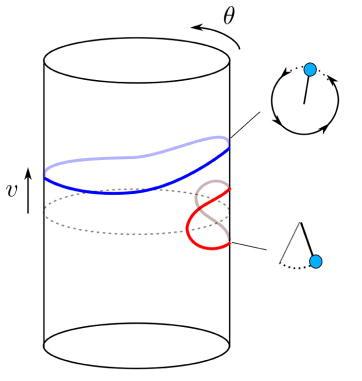
\includegraphics[width=\textwidth]{Pictures/pendo-phasespace}
		\end{center}
	\end{column}
	\begin{column}{0.5\textwidth}
 		\begin{itemize}
 			\item Consider {\bf all possible} configurations.
 			\item Collect all possible pairs of position/momentum.
 		\end{itemize}
		
		\vspace{1em}		
		\begin{defblock}[Phase Space]
			\begin{itemize}
				\item[=] collection of all \emph{states}
				\item[=] set of every possible "initial datas" (sufficient to reconstruct the motion).
			\end{itemize}
		\end{defblock}

		\vspace{1em}				
		\begin{mathblock}
			The Phase space is a \underline{symplectic} smooth manifold $(M)$.
		\end{mathblock}		
		
	\end{column}
\end{columns}
\end{frame}
\note[itemize]{
	\item You get an infinite cylinder (in the case of bipendulum I cannot picture it because we go directly into more than 2 dimensions.
	\item ho disegnato due traiettori sul fase space per mostrare come due natural motions si possono rappresentare bene qui sopra.
	\item per capire il significato di dell'aggettivo simplettico dobbiamo introdurre qualche altro interprete.

}
%-------------------------------------------------------------------------------------------------------------------------------------------------


\end{document}